\documentclass[border=3pt]{standalone}
% Preâmbulo compartilhado pelos diagramas TikZ da aula 10 de IHC (Planejamento da Avaliação)
\usepackage[T1]{fontenc}
\usepackage[utf8]{inputenc}
\usepackage{lmodern}
\usepackage{amsmath}
\usepackage{xcolor}
\usepackage{tikz}
\usetikzlibrary{arrows.meta,angles,quotes,decorations.pathmorphing,decorations.pathreplacing,calc,
                positioning,shapes.geometric,shapes.misc,backgrounds,fit,
                math}

% Paleta (mesma dos SVGs originais)
% Paleta da disciplina de IHC: acento roxo (#755099), da capa do livro.
% (o nome "dblue" é mantido para não alterar todos os diagramas)
\definecolor{dblue}{HTML}{755099}
\definecolor{dorange}{HTML}{B3541E}
\definecolor{dgreen}{HTML}{4A7C59}
\definecolor{dred}{HTML}{9C4B4B}
\definecolor{dcream}{HTML}{F4F1EA}
\definecolor{dshade}{HTML}{DDD7C9}

% Função gaussiana (não normalizada por padrão de escala visual)
\pgfmathdeclarefunction{gauss}{3}{%
  \pgfmathparse{1/(#3*sqrt(2*pi))*exp(-((#1-#2)^2)/(2*#3^2))}%
}

% Estilos comuns (prefixo d... para não colidir com chaves internas do pgf)
\tikzset{
  >={Stealth[length=2mm]},
  dguide/.style={gray!55, dashed, line width=0.4pt},
  daxis/.style={gray!60, line width=0.7pt, ->},
  dbody/.style={fill=black!3, draw=black!80, line width=1pt},
  dacc/.style={draw=dblue, line width=1pt},
  dlbl/.style={black!55, font=\small},
  dsub/.style={black!45, font=\footnotesize},
  dstate/.style={circle, draw=black!80, fill=dcream, line width=1pt,
                 minimum size=17mm, font=\large, inner sep=1pt},
  dobs/.style={circle, draw=black!80, fill=dshade, line width=1pt,
               minimum size=14mm, font=\large, inner sep=1pt},
  dbox/.style={rounded corners=2pt, draw=black!80, fill=dcream, line width=1pt,
               align=center, inner sep=6pt},
  dop/.style={circle, draw=black!80, fill=white, line width=1pt,
              minimum size=6mm, inner sep=0pt, font=\small},
  dtrans/.style={->, dblue, line width=1pt},
  dmeas/.style={->, dorange, line width=1pt},
  dcurve/.style={line width=1pt, dblue},
  dcurveb/.style={line width=1.4pt, dorange},
}

\begin{document}
\hyphenpenalty=10000 \exhyphenpenalty=10000 \tolerance=9999 \emergencystretch=3em
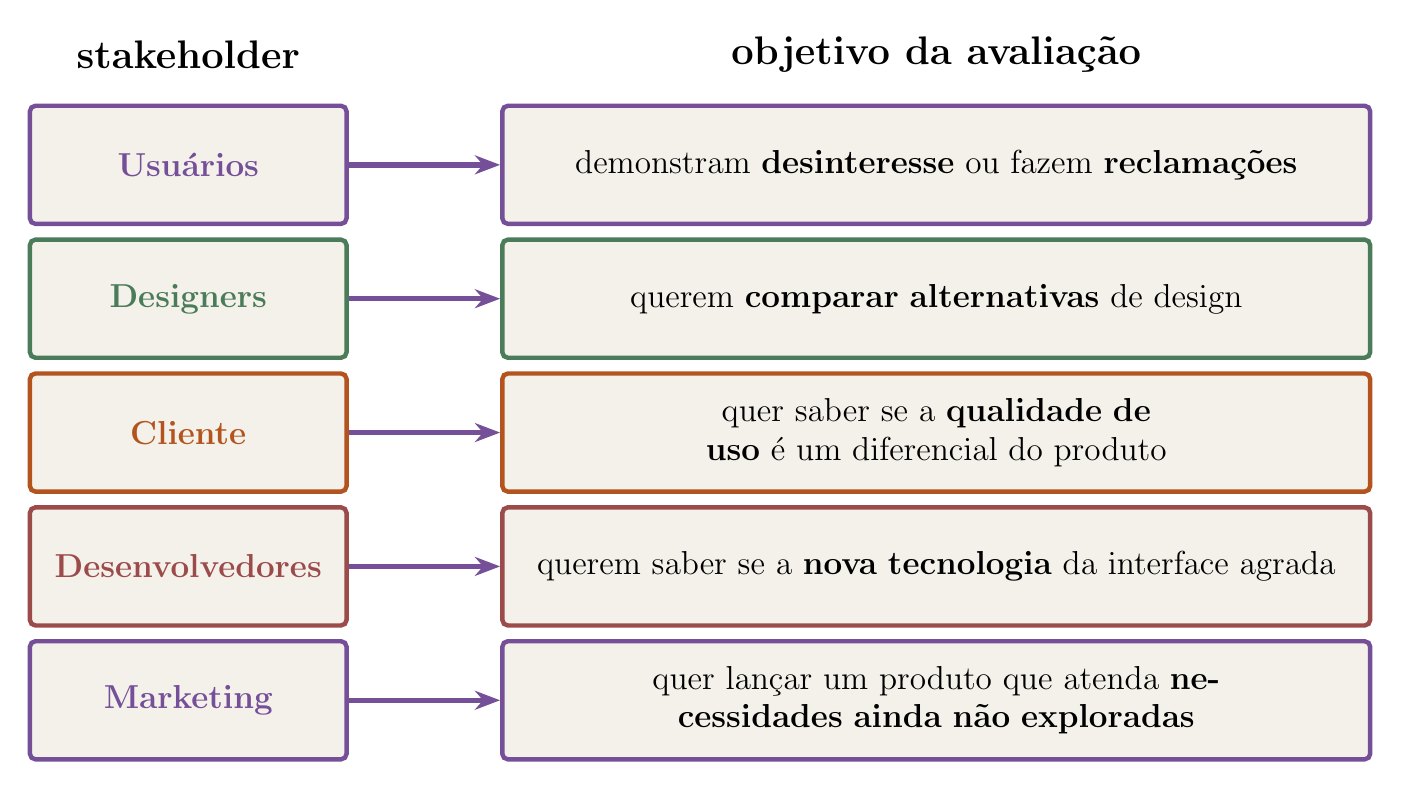
\begin{tikzpicture}[x=1cm,y=1cm]
\tikzset{s/.style={dbox, text width=3.6cm, minimum height=1.5cm, font=\large\bfseries, line width=1.6pt},
        o/.style={dbox, text width=10.6cm, minimum height=1.5cm, font=\large, line width=1.6pt}}
\foreach \y/\n/\t/\cor in {7.2/Usuários/{demonstram \textbf{desinteresse} ou fazem \textbf{reclamações}}/dblue, 5.5/Designers/{querem \textbf{comparar alternativas} de design}/dgreen, 3.8/Cliente/{quer saber se a \textbf{qualidade de uso} é um diferencial do produto}/dorange, 2.1/Desenvolvedores/{querem saber se a \textbf{nova tecnologia} da interface agrada}/dred, 0.4/Marketing/{quer lançar um produto que atenda \textbf{necessidades ainda não exploradas}}/dblue} {
  \node[s, draw=\cor] (a) at (2.4,\y) {\textcolor{\cor}{\n}};
  \node[o, draw=\cor] (b) at (11.9,\y) {\t};
  \draw[dtrans, line width=2pt, -{Stealth[length=3.2mm]}] (a.east) -- (b.west);}
\node[font=\Large\bfseries] at (2.4,8.6) {stakeholder};
\node[font=\Large\bfseries] at (11.9,8.6) {objetivo da avaliação};
\end{tikzpicture}
\end{document}
